\usetikzlibrary{decorations.markings}
\newif\iflabrev
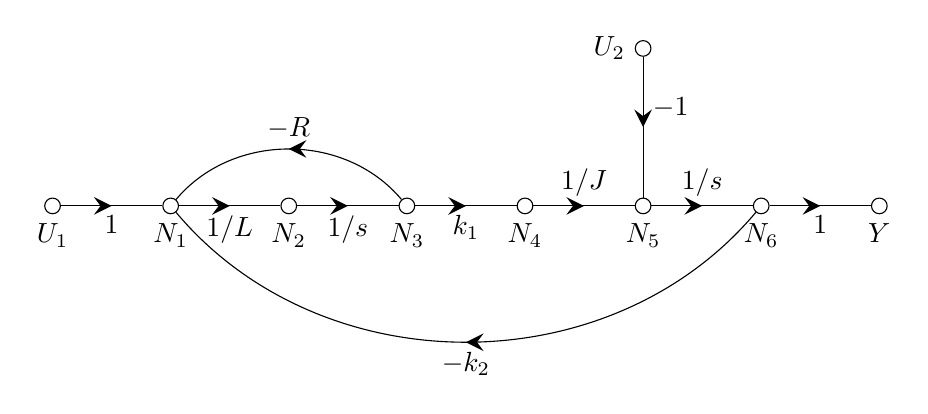
\begin{tikzpicture}
[
label revd/.is if=labrev,
amark/.style={
            decoration={             
                        markings,   
                        mark=at position {0.5} with { 
                                    \arrow[scale=2,>=stealth]{>},
                                    \iflabrev \node[above] {#1};\else \node[below] {#1};\fi
                        }
            },
            postaction={decorate}
},
terminal/.style 2 args={draw,circle,inner sep=2pt,label={#1:#2}},
]

\node[terminal={below}{$U_1$}] (a) at (0,0) {};
\node[terminal={below }{$N_1$}] (b) at (1.5cm,0) {};
\node[terminal={below}{$N_2$}] (c) at (3cm,0) {};
\node[terminal={below }{$N_3$}] (d) at (4.5cm,0) {};
\node[terminal={below }{$N_4$}] (e) at (6cm,0) {};
\node[terminal={below }{$N_5$}] (f) at (7.5cm,0) {};
\node[terminal={below }{$N_6$}] (g) at (9cm,0) {};
\node[terminal={below }{$Y$}] (h) at (10.5cm,0) {};
\node[terminal={left }{$U_2$}] (i) at (7.5cm,2cm) {};

\draw[amark=$1$] (a) to (b);
\draw[amark=$1/L$] (b) to (c);
\draw[amark=$1/s$] (c)to(d);
\draw[amark=$k_1$] (d) to (e);
\draw[amark=$1/J$,label revd] (e) to (f);
\draw[amark=$1/s$,label revd] (f) to (g);
\draw[amark=$1$] (g) to (h);
\draw[amark=$\hspace{0.7cm}-1$,label revd] (i) to (f);

\draw[amark=$-R$,label revd] (d) to[bend left=-50]  (b);
\draw[amark=$-k_2$] (g) to[bend left=50]  (b);



\end{tikzpicture}